\chapter{Measuring the Cost of Recursion}

\section{Purpose}
In this chapter, we investigate how recursive and iterative algorithms differ in their computational cost. Using the Fibonacci sequence as our case study, we’ll see how recursion can sometimes explode in complexity.

\section{The Experiment}
We designed a Python experiment that measures:
\begin{itemize}
  \item The number of function calls
  \item The number of additions
  \item The number of variable assignments
  \item The time required to compute $F_n$
\end{itemize}

\subsection{The Tracker Class}
\lstinputlisting[language=Python, caption={DataTracker and Fibonacci comparison}, label={lst:fib_analysis}]{chapters/fib_analysis.py}

\subsection{Generated Data}
After running the Python code, the script produces two files:
\begin{itemize}
  \item \texttt{fib\_results.csv} — tabular data of timing and operation counts
  \item \texttt{fib\_results\_plot.pdf} — visualization of recursive vs iterative performance
\end{itemize}

\section{Results}
\begin{figure}[H]
    \centering
    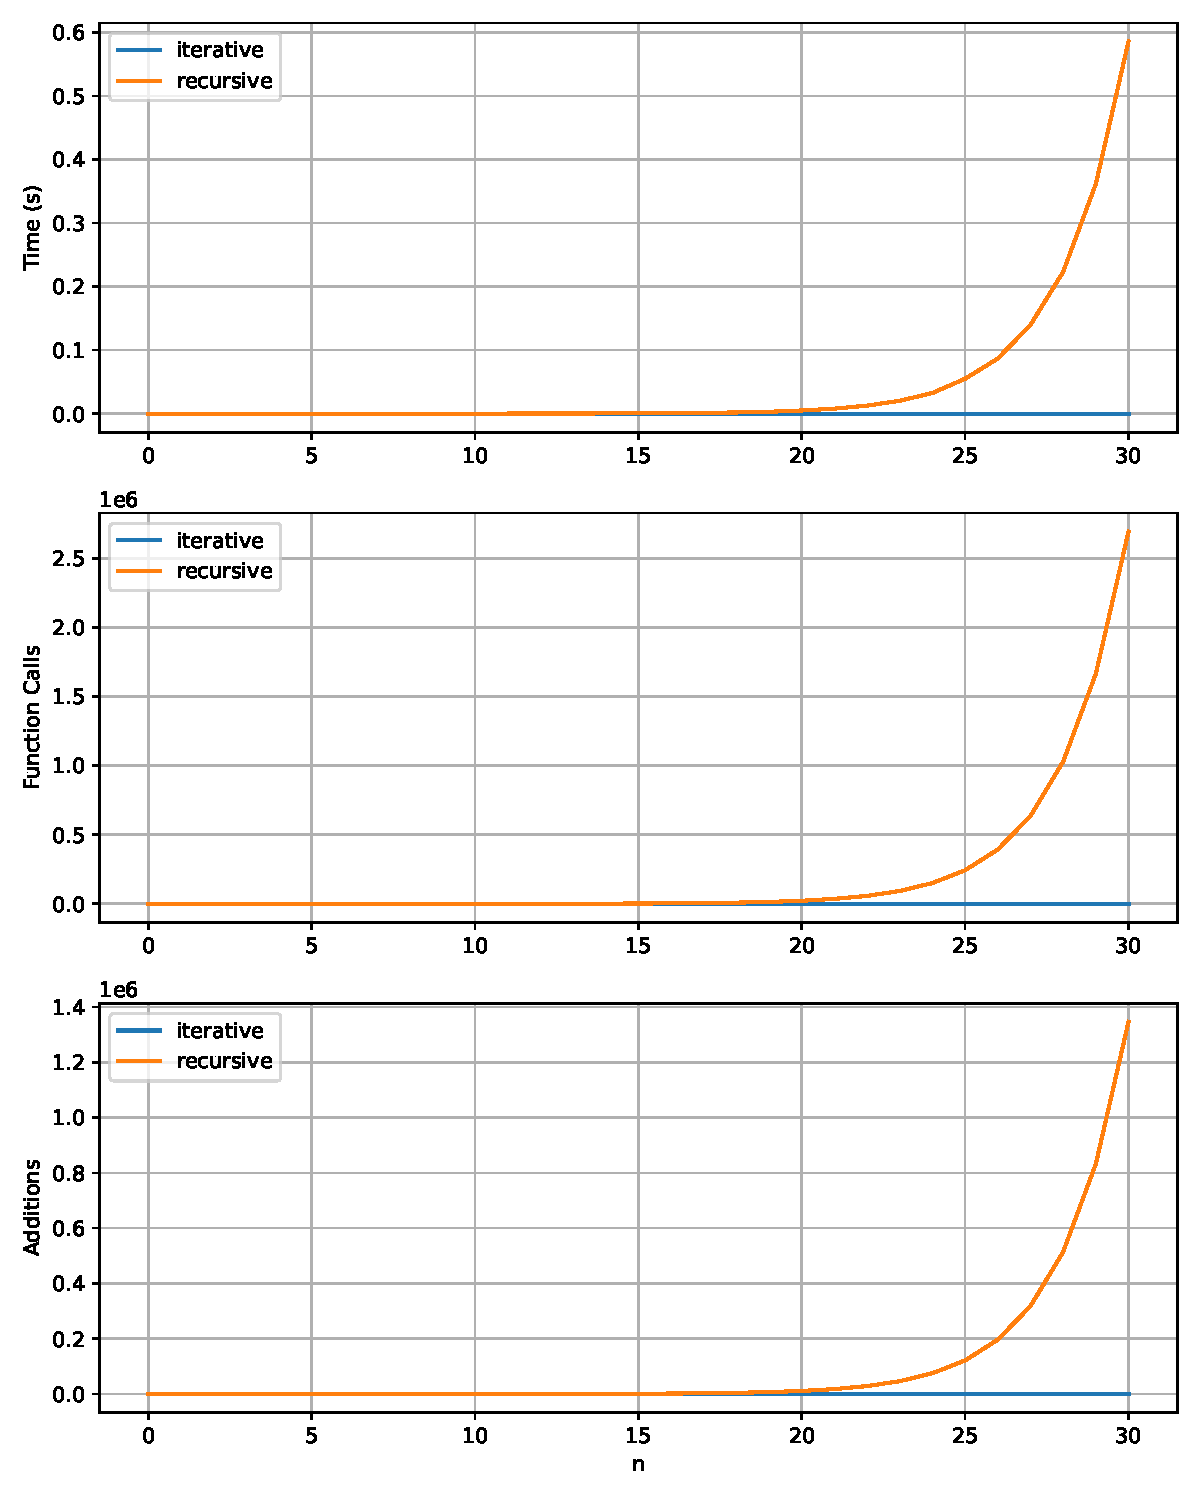
\includegraphics[width=\textwidth]{chapters/fib_results_plot.pdf}
    \caption{Recursive vs. Iterative Fibonacci performance}
\end{figure}

\section{Reflection}
Discuss:
\begin{itemize}
  \item Why does the recursive version slow down so dramatically?
  \item How might memoization or dynamic programming fix this?
  \item What do you notice about the patterns of function calls?
\end{itemize}

\section{Student Task}
Run the experiment on your own system. 
Then modify \texttt{fib\_recursive} to include memoization and compare your results.

